\documentclass[tikz, border=2pt]{standalone}
\usetikzlibrary{positioning, arrows.meta, shapes, calc, fit, babel}
\usepackage{helvet}
\renewcommand{\familydefault}{\sfdefault}
\begin{document}
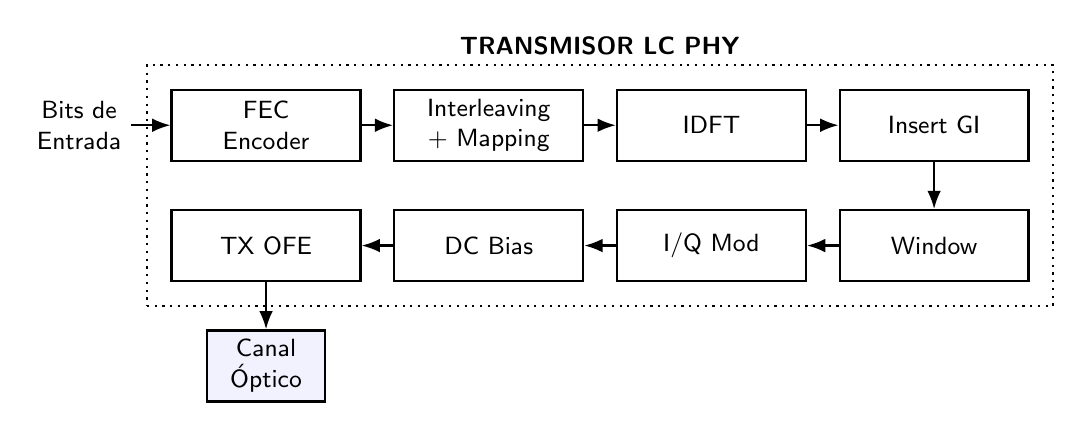
\begin{tikzpicture}[>=latex, font=\small, 
	block/.style={draw, thick, minimum height=0.9cm, minimum width=2.4cm, align=center, fill=white},
	smallblock/.style={draw, thick, minimum height=0.9cm, minimum width=1.5cm, align=center, fill=white},
	arrow/.style={-Latex, thick}]
	
	% Fila 1 (Izquierda a Derecha)
	\node[block] (fec_tx) {FEC\\Encoder};
	\node[block, right=0.4cm of fec_tx] (int_tx) {Interleaving\\+ Mapping};
	\node[block, right=0.4cm of int_tx] (idft_tx) {IDFT};
	\node[block, right=0.4cm of idft_tx] (gi_tx) {Insert GI};
	
	% Fila 2 (Derecha a Izquierda, colocada abajo)
	\node[block, below=0.6cm of gi_tx] (win_tx) {Window};
	\node[block, left=0.4cm of win_tx] (iq_tx) {I/Q Mod};
	\node[block, left=0.4cm of iq_tx] (dc_tx) {DC Bias};
	\node[block, left=0.4cm of dc_tx] (ofe_tx) {TX OFE};
	
	\node[left=0.5cm of fec_tx, align=center] (input) {Bits de\\Entrada};
	\draw[arrow] (input) -- (fec_tx);
	\draw[arrow] (fec_tx) -- (int_tx);
	\draw[arrow] (int_tx) -- (idft_tx);
	\draw[arrow] (idft_tx) -- (gi_tx);
	
	% Conexión hacia abajo de Fila 1 a Fila 2
	\draw[arrow] (gi_tx) -- (win_tx);
	
	\draw[arrow] (win_tx) -- (iq_tx);
	\draw[arrow] (iq_tx) -- (dc_tx);
	\draw[arrow] (dc_tx) -- (ofe_tx);
	
	% Canal Óptico al final de Fila 2
	\node[smallblock, below=0.6cm of ofe_tx, fill=blue!5] (channel) {Canal\\Óptico};
	\draw[arrow] (ofe_tx) -- (channel);
	
	\node[draw, dotted, thick, inner sep=0.3cm, label={above:\textbf{TRANSMISOR LC PHY}}] 
	(tx_box) [fit=(fec_tx) (gi_tx) (ofe_tx) (win_tx)] {};
\end{tikzpicture}
\end{document}
